\chapter{Congruence}
% Add: simple triangles
% Image: KA Special Triangles
Look at this picture of two geometric figures.

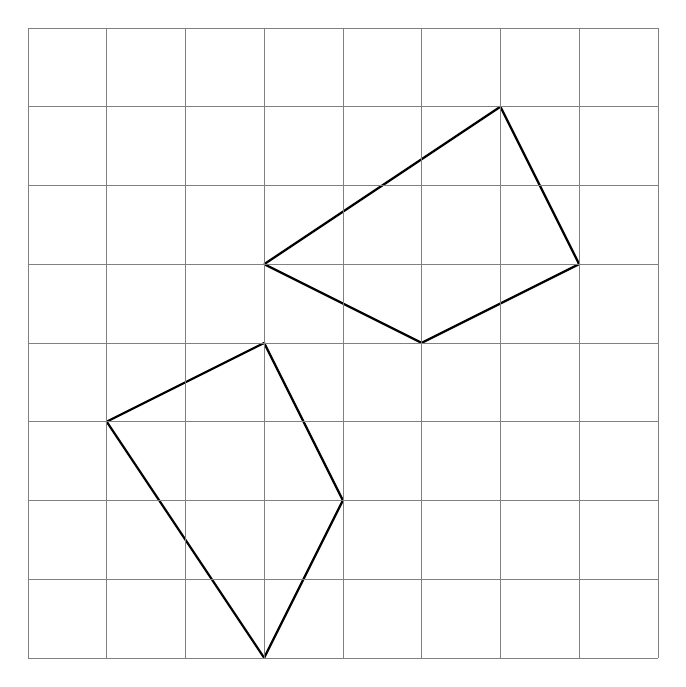
\begin{tikzpicture}
 
  	\draw [thick] (-1,-4) --  (0, -2);
	\draw [thick] (0,-2) --  (-1, 0) ;
	\draw [thick] (-1,0) --  (-3, -1); 
	\draw [thick] (-3,-1) --  (-1, -4);
	
	\draw [thick] (-1,1) --  (1, 0);
	\draw [thick] (1,0) --  (3, 1) ;
	\draw [thick] (3,1) --  (2, 3); 
	\draw [thick] (2,3) --  (-1, 1);

  \draw[help lines, step = 1cm] (-4, -4) grid (4, 4);
 
\end{tikzpicture}

They are the same shape, right? If you cut one out with scissors, it
would lay perfectly on top of the other. In geometry, we say they are
\emph{congruent}.

What is the official definition of ``congruent''? 
Two geometric figures are congruent if you can transform one into the other using
only rigid transformations. 

Which you might be wondering now, what are rigid transformations?
A transformation is \emph{Rigid} if it doesn't change the distances
between the points or the measure of the angles between the lines they
form. These are all rigid transformations:
\begin{itemize}
\item Translations
\item Rotations
\item Reflections 
\end{itemize}

Once again imagine cutting out one figure with scissors and trying to match it with the second figure, your actions are rigid transformations:
\begin{itemize}
\item Translations - sliding the cutout left and right and up and down
\item Rotations	- rotating the cutout clockwise and counterclockwise
\item Reflection - flipping the piece of paper over
\end{itemize}

A transformation is rigid if it is some combination of translations, rotations, and reflections.

\section{Triangle Congruency}

If the sides of two triangles have the same length, the triangles must be congruent:

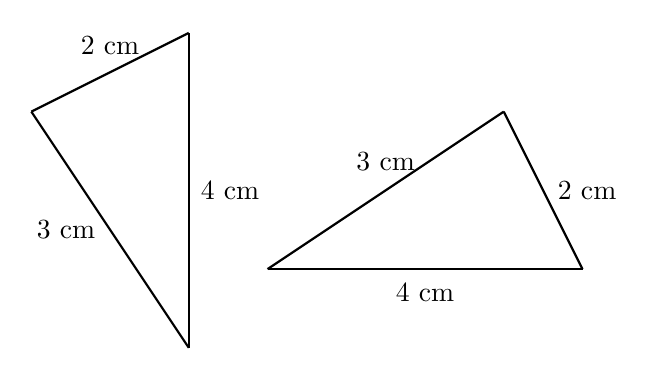
\begin{tikzpicture} 
  	\draw [thick] (-2,0) -- node[outer sep = 1pt, right]{4 cm}  (-2, 4) ;
	\draw [thick] (-2,4) --  node[outer sep = 3pt, above]{2 cm} (-4, 3); 
	\draw [thick] (-4,3) --  node[outer sep = 2pt, left]{3 cm} (-2, 0);
	
	\draw [thick] (-1,1) --  node[outer sep = 2pt, below]{4 cm}  (3, 1) ;
	\draw [thick] (3,1) --  node[outer sep = 2pt, right]{2 cm} (2, 3); 
	\draw [thick] (2,3) --  node[outer sep = 4pt, above]{3 cm} (-1, 1);
\end{tikzpicture}

To be precise, the Side-Side-Side Congruency Test says that two triangles are
congruent if three sides in one triangle are the same length as the
corresponding sides in the other. We usually refer to this as the SSS test.
% Explain with a^2 + b^2 = c^2

Note that two triangles with all three angles equal are not necessarily congruent.
For example, here are two triangles with the same interior angles, but they are
different sizes:

\begin{tikzpicture}
  \coordinate [circle, fill, inner sep=1pt] (a1) at (0,0) ;
  \coordinate [circle, fill, inner sep=1pt] (b1) at (4,0) ;
  \coordinate [circle, fill, inner sep=1pt] (c1) at (3,2) ;
  
   \coordinate [circle, fill, inner sep=1pt] (a2) at (5,0) ;
  \coordinate [circle, fill, inner sep=1pt] (b2) at (11,0) ;
  \coordinate [circle, fill, inner sep=1pt] (c2) at (9.5,3) ;
        \draw (a1) --   (b1);
        \draw (b1) -- (c1);
        \draw (c1)--  (a1);
        \pic [draw, "$63^\circ$", angle eccentricity=1.5] {angle = c1--b1--a1};
        \pic [draw, "$34^\circ$", angle eccentricity=2.0] {angle = b1--a1--c1};
        \pic [draw, "$83^\circ$", angle eccentricity=1.5] {angle = a1--c1--b1};

       \draw (a2) --  (b2);
        \draw (b2) -- (c2);
        \draw (c2)--  (a2);
        \pic [draw, "$63^\circ$", angle eccentricity=1.5] {angle = c2--b2--a2};
        \pic [draw, "$34^\circ$", angle eccentricity=2.0] {angle = b2--a2--c2};
        \pic [draw, "$83^\circ$", angle eccentricity=1.5] {angle = a2--c2--b2};

\end{tikzpicture}

These triangles are not congruent, but they are \emph{similar}. Meaning
 they have the same shape, but are not necessarily the same
size.

Therefore, if you know two angles of a triangle, you can calculate the third. So it makes sense
to say ``If two triangles have two angles that are equal, they are
similar triangles.''  And if two similar triangles have one side that
is equal in length, they must be the same size -- so they are
congruent. Thus, the Side-Angle-Angle Congruency Test says that
two triangles are congruent if two angles and side match.

What if you know that two triangles have two sides that are the same
length and that the angle between them is also equal?

\begin{tikzpicture}
  \coordinate [circle, fill, inner sep=1pt] (a1) at (0,0) ;
  \coordinate [circle, fill, inner sep=1pt] (b1) at (4,0) ;
  \coordinate [circle, fill, inner sep=1pt] (c1) at (3,2) ;
  
  \coordinate [circle, fill, inner sep=1pt] (a2) at (5,0) ;
  \coordinate [circle, fill, inner sep=1pt] (b2) at (9,0) ;
  \coordinate [circle, fill, inner sep=1pt] (c2) at (8,2) ;
  
  \draw (a1) --  node[outer sep = 0.5pt, below]{4}  (b1);
  \draw [dashed] (b1) -- (c1);
  \draw (c1)--  node[outer sep = 5pt, above]{3.5} (a1);
  \pic [draw, "$34^\circ$", angle eccentricity=2.0] {angle = b1--a1--c1};

  \draw (a2) --  node[outer sep = 0.5pt, below]{4}  (b2);
  \draw [dashed] (b2) -- (c2);
  \draw (c2)--  node[outer sep = 5pt, above]{3.5} (a2);
  \pic [draw, "$34^\circ$", angle eccentricity=2.0] {angle = b2--a2--c2};
\end{tikzpicture}

Yes, they must be congruent. This is the Side-Angle-Size Congruency Test.

What if the angle isn't the one between the two known sides? If it is
a right angle, you can be certain the two triangles are congruent.
(How do I know? Because the Pythagorean Theorem tells us that we can
calculate the length of the third side. There is only one possibility,
thus all three sides must be the same length.)

\begin{tikzpicture}
  \coordinate [circle, fill, inner sep=1pt] (a1) at (0,0) ;
  \coordinate [circle, fill, inner sep=1pt] (b1) at (4,0) ;
  \coordinate [circle, fill, inner sep=1pt] (c1) at (4,2) ;
  
   \coordinate [circle, fill, inner sep=1pt] (a2) at (5,0) ;
  \coordinate [circle, fill, inner sep=1pt] (b2) at (9,0) ;
  \coordinate [circle, fill, inner sep=1pt] (c2) at (9,2) ;
        \draw (a1) --  node[outer sep = 0.5pt, below]{3.5}  (b1);
        \draw [dashed] (b1) -- (c1);
        \draw (c1)--  node[outer sep = 5pt, above]{4} (a1);
        \pic [draw] {right angle = a1--b1--c1};

        \draw (a2) --  node[outer sep = 0.5pt, below]{3.5}  (b2);
        \draw [dashed] (b2) -- (c2);
        \draw (c2)--  node[outer sep = 5pt, above]{4} (a2);
        \pic [draw] {right angle = a2--b2--c2};
\end{tikzpicture}

In this case, the third side of each triangle must be $\sqrt{4^2 - 3.5^2} \approx 1.9$.

What if the know angle is less than $90^\circ$? \emph{The triangles
  are not necessarily congruent.} For example, lets say that there are
two triangles with sides of length 5 and 7 and that the corresponding
angle (at the end of the side of length 7) on each is $45^\circ$. Two
different triangles satisfy this:

\begin{tikzpicture}
  \coordinate [circle, fill, inner sep=1pt] (a1) at (0,0) ;
  \coordinate [circle, fill, inner sep=1pt] (b1) at (7,0) ;
  \coordinate [circle, fill, inner sep=1pt] (c1) at (4,3) ;
  \coordinate [circle, fill, inner sep=1pt] (a2) at (8,0) ;
  \coordinate [circle, fill, inner sep=1pt] (b2) at (15,0) ;
  \coordinate [circle, fill, inner sep=1pt] (c2) at (11,4) ;
  \draw (a1) --  node[outer sep = 0.5pt, below]{7}  (b1);
  \draw [dashed] (b1) -- (c1);
  \draw (c1)--  node[outer sep = 5pt, above]{5}(a1);
  \pic [draw, "$45^\circ$", angle eccentricity=1.5] {angle = c1--b1--a1};
  \draw (a2) --  node[outer sep = 0.5pt, below]{7}  (b2);
  \draw [dashed] (b2) -- (c2);
  \draw (c2)--  node[outer sep = 5pt, above]{5} (a2);
  \pic [draw, "$45^\circ$", angle eccentricity=1.5] {angle = c2--b2--a2};
\end{tikzpicture}

Let's see this another way by laying one triangle on top of the other:

\begin{tikzpicture}
  \coordinate [circle, fill, inner sep=1pt] (a1) at (0,0) ;
  \coordinate [circle, fill, inner sep=1pt] (b1) at (7,0) ;
  \coordinate [circle, fill, inner sep=1pt] (c1) at (4,3) ;
  \coordinate [circle, fill, inner sep=1pt] (c2) at (3,4) ;
  \coordinate (d) at (2,5);
  \coordinate (e) at (3.5,3.5);

  \draw (a1) --  node[outer sep = 0.5pt, below]{7}  (b1);
  \draw [dashed,->] (b1) -- (d);
  \draw [dashed] (a1) -- (e);
  \draw (c1)--  node[outer sep = 5pt, below]{5}(a1);
  \draw (c2)--  node[outer sep = 5pt, above]{5}(a1);
  \pic [draw, "$45^\circ$", angle eccentricity=1.5] {angle = c1--b1--a1};
   \pic [draw, angle radius=8] {right angle = b1--e--a1};
\end{tikzpicture}


So there is \emph{not} a general Side-Side-Angle Congruency Test.

Here, then, is the list of common congruency tests:
\begin{itemize}
\item Side-Side-Side: All three sides have the same measure
\item Side-Angle-Angle: Two angles and one side have the same measure
\item Side-Angle-Side: Two sides and the angle between them have the same measure
\item Side-Side-Right: They are right triangles and two sides have the same measure
\end{itemize}

\begin{Exercise}[title={Congruent Triangles}, label=con_triangles]
  Ted is terrible at drawing triangles: he always draws them exactly
  the same. Fortunately, he has marked these diagrams with the sides
  and angles that he measured. For each pair of triangles, write if
  you know them to be congruent and which congruency test proves
  it. For example:

\begin{tikzpicture}[scale=0.7]
  \coordinate [circle, fill, inner sep=1pt] (a1) at (0,1) ;
  \coordinate [circle, fill, inner sep=1pt] (b1) at (5,0) ;
  \coordinate [circle, fill, inner sep=1pt] (c1) at (4,2) ;
  
  \coordinate [circle, fill, inner sep=1pt] (a2) at (6,1) ;
  \coordinate [circle, fill, inner sep=1pt] (b2) at (11,0) ;
  \coordinate [circle, fill, inner sep=1pt] (c2) at (10,2) ;
  \draw (a1) --  node[outer sep = 0.5pt, below]{3.5}  (b1);
  \draw (b1) -- node[outer sep = 2pt, right]{4} (c1);
  \draw (c1)--  node[outer sep = 2pt, above]{} (a1);
  \pic [draw,  "$120^\circ$", angle eccentricity=2.0] {angle = c1--b1--a1};

  \draw (a2) --  node[outer sep = 0.5pt, below]{3.5}  (b2);
  \draw  (b2) -- node[outer sep = 2pt, right]{4} (c2);
  \draw (c2) -- node[outer sep = 2pt, above]{} (a2);
  \pic [draw,  "$120^\circ$",, angle eccentricity=2.0] {angle = c2--b2--a2};
\end{tikzpicture}

  (These drawings are clearly not accurate, but you are told the measurements are.) The answer is ``Congruent by the Side-Angle-Side test.''

  \begin{multicols}{2}

\begin{tikzpicture}[scale=0.6]
  \coordinate [circle, fill, inner sep=1pt] (a1) at (0,1) ;
  \coordinate [circle, fill, inner sep=1pt] (b1) at (5,0) ;
  \coordinate [circle, fill, inner sep=1pt] (c1) at (4,2) ;
  
  \coordinate [circle, fill, inner sep=1pt] (a2) at (6,1) ;
  \coordinate [circle, fill, inner sep=1pt] (b2) at (11,0) ;
  \coordinate [circle, fill, inner sep=1pt] (c2) at (10,2) ;
  \draw (a1) --  node[outer sep = 0.5pt, below]{3.5}  (b1);
  \draw (b1) -- node[outer sep = 2pt, right]{} (c1);
  \draw (c1)--  node[outer sep = 2pt, above]{6} (a1);
  \pic [draw,  "$90^\circ$", angle eccentricity=2.0] {angle = c1--b1--a1};

  \draw (a2) --  node[outer sep = 0.5pt, below]{3.5}  (b2);
  \draw  (b2) -- node[outer sep = 2pt, right]{} (c2);
  \draw (c2) -- node[outer sep = 2pt, above]{6} (a2);
  \pic [draw,  "$90^\circ$",, angle eccentricity=2.0] {angle = c2--b2--a2};
\end{tikzpicture}

\hspace{3cm}

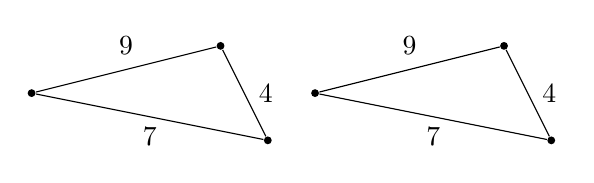
\begin{tikzpicture}[scale=0.6]
  \coordinate [circle, fill, inner sep=1pt] (a1) at (0,1) ;
  \coordinate [circle, fill, inner sep=1pt] (b1) at (5,0) ;
  \coordinate [circle, fill, inner sep=1pt] (c1) at (4,2) ;
  
  \coordinate [circle, fill, inner sep=1pt] (a2) at (6,1) ;
  \coordinate [circle, fill, inner sep=1pt] (b2) at (11,0) ;
  \coordinate [circle, fill, inner sep=1pt] (c2) at (10,2) ;
  \draw (a1) --  node[outer sep = 0.5pt, below]{7}  (b1);
  \draw (b1) -- node[outer sep = 2pt, right]{4} (c1);
  \draw (c1)--  node[outer sep = 2pt, above]{9} (a1);

  \draw (a2) --  node[outer sep = 0.5pt, below]{7}  (b2);
  \draw  (b2) -- node[outer sep = 2pt, right]{4} (c2);
  \draw (c2) -- node[outer sep = 2pt, above]{9} (a2);
\end{tikzpicture}


\begin{tikzpicture}[scale=0.6]
  \coordinate [circle, fill, inner sep=1pt] (a1) at (0,1) ;
  \coordinate [circle, fill, inner sep=1pt] (b1) at (5,0) ;
  \coordinate [circle, fill, inner sep=1pt] (c1) at (4,2) ;
  
  \coordinate [circle, fill, inner sep=1pt] (a2) at (6,1) ;
  \coordinate [circle, fill, inner sep=1pt] (b2) at (11,0) ;
  \coordinate [circle, fill, inner sep=1pt] (c2) at (10,2) ;
  \draw (a1) --  node[outer sep = 0.5pt, below]{7}  (b1);
  \draw (b1) -- node[outer sep = 2pt, right]{} (c1);
  \draw (c1)--  node[outer sep = 2pt, above]{} (a1);
  \pic [draw,  "$35^\circ$",, angle eccentricity=2.0] {angle = c1--b1--a1};
  \pic [draw,  "$62^\circ$",, angle eccentricity=2.0] {angle = b1--a1--c1};

  \draw (a2) --  node[outer sep = 0.5pt, below]{7}  (b2);
  \draw  (b2) -- node[outer sep = 2pt, right]{} (c2);
  \draw (c2) -- node[outer sep = 2pt, above]{} (a2);
  \pic [draw,  "$35^\circ$",, angle eccentricity=2.0] {angle = c2--b2--a2};
  \pic [draw,  "$62^\circ$",, angle eccentricity=2.0] {angle = b2--a2--c2};

\end{tikzpicture}

\hspace{3cm}


\begin{tikzpicture}[scale=0.6]
  \coordinate [circle, fill, inner sep=1pt] (a1) at (0,1) ;
  \coordinate [circle, fill, inner sep=1pt] (b1) at (5,0) ;
  \coordinate [circle, fill, inner sep=1pt] (c1) at (4,2) ;
  
  \coordinate [circle, fill, inner sep=1pt] (a2) at (6,1) ;
  \coordinate [circle, fill, inner sep=1pt] (b2) at (11,0) ;
  \coordinate [circle, fill, inner sep=1pt] (c2) at (10,2) ;
  \draw (a1) --  node[outer sep = 0.5pt, below]{8}  (b1);
  \draw (b1) -- node[outer sep = 2pt, right]{6} (c1);
  \draw (c1)--  node[outer sep = 2pt, above]{} (a1);
  \pic [draw,  "$28^\circ$",, angle eccentricity=2.0] {angle = b1--a1--c1};

  \draw (a2) --  node[outer sep = 0.5pt, below]{8}  (b2);
  \draw  (b2) -- node[outer sep = 2pt, right]{6} (c2);
  \draw (c2) -- node[outer sep = 2pt, above]{} (a2);
  \pic [draw,  "$28^\circ$",, angle eccentricity=2.0] {angle = b2--a2--c2};

\end{tikzpicture}


\end{multicols}
\end{Exercise}

\begin{Answer}[ref=con_triangles]
\begin{multicols}{2}
Congruent by the Side-Side-Right Congruency Test.

Congruent by the Side-Side-Side Congruency Test.

Congruent by the Side-Angle-Angle Congruency Test.

We don't know if they are congruent. The measured angle is not between the measured sides.

% Image: Congruence Cheat Sheat
\end{multicols}

\end{Answer}



